%% ------------------------------------------------------------------------- %%
\chapter{Programação Dinâmica}
\label{cap:programacao-dinamica}

\section{Introdução}

Neste capítulo apresentaremos o primeiro algoritmo realmente eficiente para calcular o \LCA\ entre dois vértices em uma árvore enraizada utilizando programação dinâmica. Este algoritmo terá complexidade de tempo $O(log(n))$ por consulta, onde $log(n)$ é o logaritmo na base 2 de $n$ - a quantidade de vértices na árvore.

\section{Descrição}

A ideia deste algoritmo segue a mesma dos capítulos anteriores: primeiro são pré-calculados ancestrais dos vértices para depois realizar as consultas.

Para cada vértice serão pré-computados os ancestrais cuja profundidade na árvore é menor do que a sua em uma potência de dois - ou seja - 1, 2, 4, 8, ... , $h$ níveis acima dele, onde $h$ é a maior potência de dois que não ultrapasse a altura da árvore. Em outras palavras, para cada vértice serão pré-calculados até $log(n)$ ancestrais diferentes.

Para ilustrar este pré-processamento, introduzimos a figura a seguir:

\begin{figure}[htb]
\begin{center}
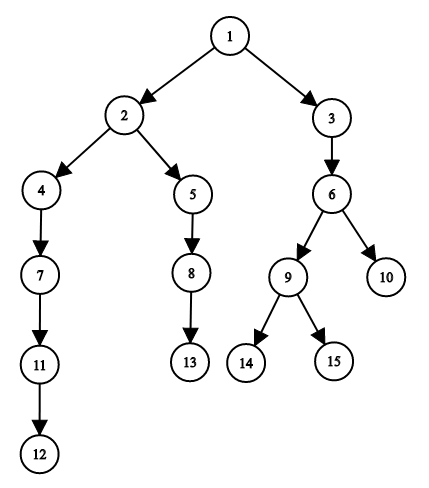
\includegraphics[width=7.2cm]{images/graph_dp.png}
\end{center}
\caption{\label{fig:arvore-6}Árvore enraizada de altura 6.}
\end{figure}

Após o pré-processamento, teríamos como os ancestrais, para os vértices 12 e 15:

\begin{itemize}
    \item Vértice 11

    \begin{table}[htb]
    \centering
    \begin{tabular}{|l|c|c|c|c|c|c|c|c|c|c|c|c|c|c|}
    \hline
    Altura relativa & -1 & -2 & -4 \\ \hline
    Ancestral       & 7 & 4  & 1 \\ \hline
    \end{tabular}
    \caption{Ancestrais relativos do vértice 12}
    \end{table}
    
    \item Vértice 15
    
    \begin{table}[htb]
    \centering
    \begin{tabular}{|l|c|c|c|c|c|c|c|c|c|c|c|c|c|c|}
    \hline
    Altura relativa & -1 & -2 & -4 \\ \hline
    Ancestral       & 9  & 6  & 1 \\ \hline
    \end{tabular}
    \caption{Ancestrais relativos do vértice 15}
    \end{table}

\end{itemize}

Por conveniência, a partir de agora vamos nos referir a cada ancestral de um vértice $v$ como $ancestral_v(2^i)$ para todo inteiro $i$.

Agora, para calcular o \LCA\ entre dois vértices $a$ e $b$ faremos o que já vimos em todos os capítulos anteriores: vamos caminhar até a raiz com ambos. A maneira que faremos isso desta vez é dando pulos de tamanho "potência de dois"\  com auxílio dos valores que já foram pré-computados. Além disso, cada pulo é de um tamanho diferente.

Vamos assumir sem perda de generalidade que $b$ é mais profundo do que $a$. Inicialmente, são feitos sucessivos pulos suficientes para que $a$ e $b$ estejam exatamente no mesmo nível. Por exemplo, se a profundidade de $a$ é 3 e a de $b$ é 6, devemos subir $b$ em $6 - 3 = 3$ níveis: o que equivale a um pulo de tamanho 2 e um pulo de tamanho 1. Provaremos adiante que sempre conseguimos igualar os níveis dos vértices dando pulos diferentes de tamanho de alguma potência de dois cada.

Tendo $a$ e $b$ agora no mesmo nível, podemos checar se eles são iguais. Se forem, isso significa que $a$ estava originalmente no caminho de $b$ até a raiz e que portanto ela é o \LCA. Caso contrário, devemos encontrar o maior tamanho de um pulo para subir simultaneamente os vértices $a$ e $b$ de forma que ainda sejam diferentes. Encontraremos este valor dando pulos distintos de tamanho de alguma potência de dois. A figura a seguir um possível cenário:

\begin{figure}[htb]
\begin{center}
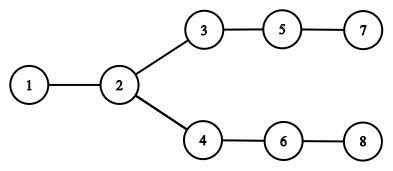
\includegraphics{images/graph_dp2.png}
\end{center}
\caption{\label{fig:arvore-5}Árvore enraizada de altura 5.}
\end{figure}


Consideremos $a = 7$ e $b = 8$. Vamos listar os possíveis valores a serem escolhidos para subir simultaneamente $a$ e $b$. Note que ao subir $2^3 = 8$ ou mais níveis a restrição da altura máxima da árvore seria violada, e por isso a última potência de dois a ser considerada é $2^2 = 4$.

\begin{itemize}
    \item \textbf{4}: Ao subir 4 níveis, $a$ e $b$ são iguais (ambos = $1$). Não o fazemos.
    \item \textbf{2}: Ao subir 2 níveis, $a$ e $b$ são diferentes. Então atualizamos $a$ e $b$ para tais ancestrais. Agora $a = 3$ e $b = 4$
    \item \textbf{1}: Ao subir 1 nível, os valores atualizados de $a$ e $b$ são iguais (ambos = $2$). Não o fazemos.
\end{itemize}

Em outras palavras, o que encontramos são os dois vértices distintos mais próximos à raiz que contêm, respectivamente, os vértices $a$ e $b$ em suas sub-árvores. Assim, o pai destes vértices será o \LCA\, já que será o primeiro vértice que contém ambos $a$ e $b$ em sua sub-árvore.

\vspace{1cm}

Voltando à figura \ref{fig:arvore-6}, vamos simular os passos completos para encontrar o \LCA(12, 15):

\begin{itemize}
    \item Vértices 12 e 15 não estão na mesma altura. O vértice 12 é mais profundo, então vamos subi-lo em direção à raiz.
    \item A diferença das profundidades de 12 e 15 é de um. Então agora seu novo valor é $ancestral_{12}(1) =$ vértice 11.
    \item Agora, vamos determinar qual é o o maior inteiro $i$ tal que $ancestral_{11}(i) \neq ancestral_{15}(i)$. Testando as potências de dois, da maior para a menor, tentaremos primeiro subir 4 níveis - o que resultaria em ambos irem até o vértice $1$. Então, testamos 2 níveis - o que resulta nos vértices $4$ e $6$, respectivamente. Como são distintos, vamos para eles. Finalmente, tentamos subir 1 nível - o que resulta nos vértices $2$ e $3$ - ainda distintos. Vamos para eles.
    \item Finalmente, sabemos que os últimos dois vértices antes do \LCA\ são $2$ e $3$, então basta retornar o pai de qualquer um deles para obter o \LCA: o vértice $1$.
\end{itemize}


\vspace{10cm}

\section{Algoritmo}

Vamos dividir nosso algoritmo em duas partes: pré-processamento da matriz de programação dinâmica e a função de obtenção do \LCA\ entre dois vértices $a$ e $b$.

Como explicado na seção 5.2, vamos calcular os ancestrais de "potência de dois"\ de cada vértice da árvore. Assim, $pd[i][j]$ representa o ancestral $2^j$ do vértice $i$.

\vspace{0.5cm}

Primeiro, para o pré-processamento, vamos apresentar a seguinte recorrência:

\begin{center}
  pd[i][j]=\begin{cases}
    pai[i], & \text{se $j = 0$}.\\
    pd[pd[i][j-1]][j-1], & \text{caso contrário}.
  \end{cases}
\end{center}

\vspace{0.2cm}

Segue o código que preenche a matriz $pd$ linha a linha:

\begin{algorithm}[H]
\caption{Cálculo da matriz de programação dinâmica ($pd$)}
\begin{algorithmic}[1]
\Function{\textsc{CalculaAncestrais}}{}
    \For{cada $nivel$ em $logNiveis$}
        \For{cada $vertice$ em $vertices$}
            \If{$nivel = 0$}
                \State $pd[vertice][nivel] \rec pai[vertice]$
            \Else
                \State $pd[vertice][nivel] \rec pd[pd[vertice][nivel-1]][nivel-1]$
            \EndIf
        \EndFor
    \EndFor
\EndFunction
\end{algorithmic}
\end{algorithm}

Feito isso, agora podemos escrever o código que responderá as consultas de \LCA\ entre dois vértices $a$ e $b$:

\vspace{0.2cm}

\begin{algorithm}[H]
\caption{Obtenção do \LCA}
\begin{algorithmic}[1]
\Function{\textsc{LCA\_PD}}{a,\ b}
    \If{$prof[b] < prof[a]$}
        \State $troca(a, b)$
    \EndIf
    \State $bAtual \rec b$
    \State $i \rec logNiveis$
    \While { $i \geq 0$}
        \If{$prof[bAtual] - 2^i \geq prof[a]$}
            \State $bAtual \rec pd[b][i]$
        \EndIf
        \vspace{-0.2cm}
        \State $i \rec i - 1$
    \EndWhile
    \State $b \rec bAtual$
    \If{$a = b$}
        \\\hspace{11mm} \Return $a$
    \EndIf
    \State $i \rec logNiveis$
    \While { $i \geq 0$}
        \If{$pd[a][i] \neq pd[b][i]$}
            \State $a \rec pd[a][i]$
            \State $b \rec pd[b][i]$
        \EndIf
        \vspace{-0.2cm}
        \State $i \rec i - 1$
    \EndWhile
    \\\hspace{5mm} \Return $pai[a]$
\EndFunction
\end{algorithmic}
\end{algorithm}

\vspace{10cm}

\section{Corretude}

\subsection{Pré-processamento}

Neste algoritmo é feito o pré-processamento da recorrência apresentada na seção 5.3.

Na primeira iteração do laço mais externo são calculados os $ancestrais\ 2^0$ de cada vértice (o caso base da recorrência). Note que tal ancestral é seu pai imediato, então podemos facilmente determinar $pd[x][0]$ para todo vértice $x$. Isto é feito na linha 5 do código.

Em seguida, da segunda iteração em diante do laço mais externo são obtidos os ancestrais "não diretos"\ (isto é, um ancestral que não é o pai imediato de um nó). Podemos notar que $ancestral\ 2^i$ de um vértice $v$ é o $ancestral\ 2^{i-1}$ do $ancestral\ 2^{i-1}$ de $v$. Afinal, $2^{i-1} + 2^{i-1} = 2^i$, e por este motivo podemos fazer com que no caminho de um vértice até o seu ancestral em questão visitemos este vértice intermediário. Então, concluímos que a linha 7 produz o resultado correto de $pd[vertice][nivel]$, já que todos os ancestrais $nivel - 1$ já foram computados e só dependemos deles nesta etapa.


\subsection{LCA}

Agora vamos analisar a corretude do algoritmo de obtenção do \LCA\ baseado nos valores pré-computados durante a execução do algoritmo 6.

Nas linhas 2 e 3 os vértices $a$ e $b$ são trocados caso o vértice $a$ seja mais profundo. O motivo disso é que queremos assumir que a profundidade do vértice $b$ sempre seja maior ou igual do que a profundidade do vértice $a$.

No laço da linha 5 percorremos o caminho do vértice $b$ até a raiz, subindo este vértice até o nó de seu caminho cuja profundidade seja a mesma do vértice $a$. Sendo $logNiveis$ o valor do $log$ da altura da árvore, percorremos este laço de maneira decrescente começando em $logNiveis$. Nas linhas 6 e 7 atualizamos o valor atual do vértice $b$ caso ao subir $2^i$ níveis a profundidade do novo nó obtido não é menor do que a do vértice $a$ - afinal, queremos garantir que no final do laço ambos estejam no mesmo nível. Como qualquer número inteiro pode ser representado como uma soma de potências de dois, garantimos que ao final da iteração teremos conseguido com que $profundidade[b] = profundidade[a]$.

Nas linhas 9 e 10 é verificado se $a = b$. Como $a$ e $b$ agora estão na mesma altura da árvore, eles podem coincidir (ou seja, $b$ estava na subárvore de $a$) - concluindo que obtivemos o \LCA\ e podemos parar o algoritmo.

Caso a execução do código alcance a linha 11, sabemos então que $a$ e $b$ ainda não se encontraram (e portanto ainda não sabemos quem é o \LCA). No laço da linha 11 iteramos de $logNiveis$ até 0 para verificar todos os $ancestrais\ 2^i$ de $a$ e $b$ em ordem decrescente. Na linha 12 é verificado se $ancestral_a\ 2^i$ difere de $ancestral_b\ 2^i$. Caso isso se confirme, sabemos que se for dado um pulo de tamanho $2^i$ ainda não teremos encontrado o \LCA, já que se se tais ancestrais fossem iguais poderíamos ter encontrado o \LCA\ ou qualquer vértice acima do \LCA\ no caminho da raiz. Então, atualizamos ambos $a$ e $b$ para seus respectivos ancestrais e repetimos isso até o laço acabar. No final deste laço saberemos que $a$ e $b$ estarão nos vértices menos profundos dos seus caminhos até a raiz que ainda não são o \LCA\ entre eles (pelo mesmo argumento de que conseguimos chegar em qualquer altura dando pulos de tamanho potência de dois). Assim, basta retornar o pai de qualquer um deles que este será o \LCA\ de fato.

\vspace{10cm}

\section{Complexidade}

No pré-processamento são executados dois laços encadeados: o mais externo executa $log\ h$ iterações, onde $h$ é a altura da árvore. O laço interno executa $n$ iterações, onde $n$ é a quantidade de vértices da árvore. Assim, como no pior caso $h = n$, concluímos que a função $CalculaAncestrais$ tem complexidade de tempo e de memória ambos $O(n\ log\ n)$.

No cálculo do \LCA\ fazemos operações de tempo constante nas linhas 2, 3 e 4. Os laços das linhas 5 e 11 ambos executam $log\ h$ iterações cada, com $h$ sendo a altura da árvore, e em cada iteração são feitas operações de tempo constante. Novamente, como no pior caso $h$ é igual ao número $n$ de vértices na árvore, concluimos que a função $LCA\_PD$ possui complexidade de tempo $O(log\ n)$.